%!TEX root = ../../thesis.tex
\section{Oscillators}
\label{sec:webaudio-osc}

\begin{quote}
  ``It's basic elements, like love, dancing and sine waves.'' -
  Eero Johannes (We call it Skweee)
\end{quote}

Oscillators in physics, and generally in the analog world, are devices that generate and form electronic signals. When they are wired together with speakers and produce frequencies within the human range of hearing (20Hz to 20kHz), they can be used to create electronic sounds. Depending on the type of wave that is used as an initial signal and the signal's frequency, sounds are softer, harder, higher (high frequency) or lower (low frequency). Oscillators build the foundation of electronic music production and they are the building blocks for many instruments (e.g. synthesizers) and techniques (e.g. LFO).

\begin{figure}[htb]
  \centerline{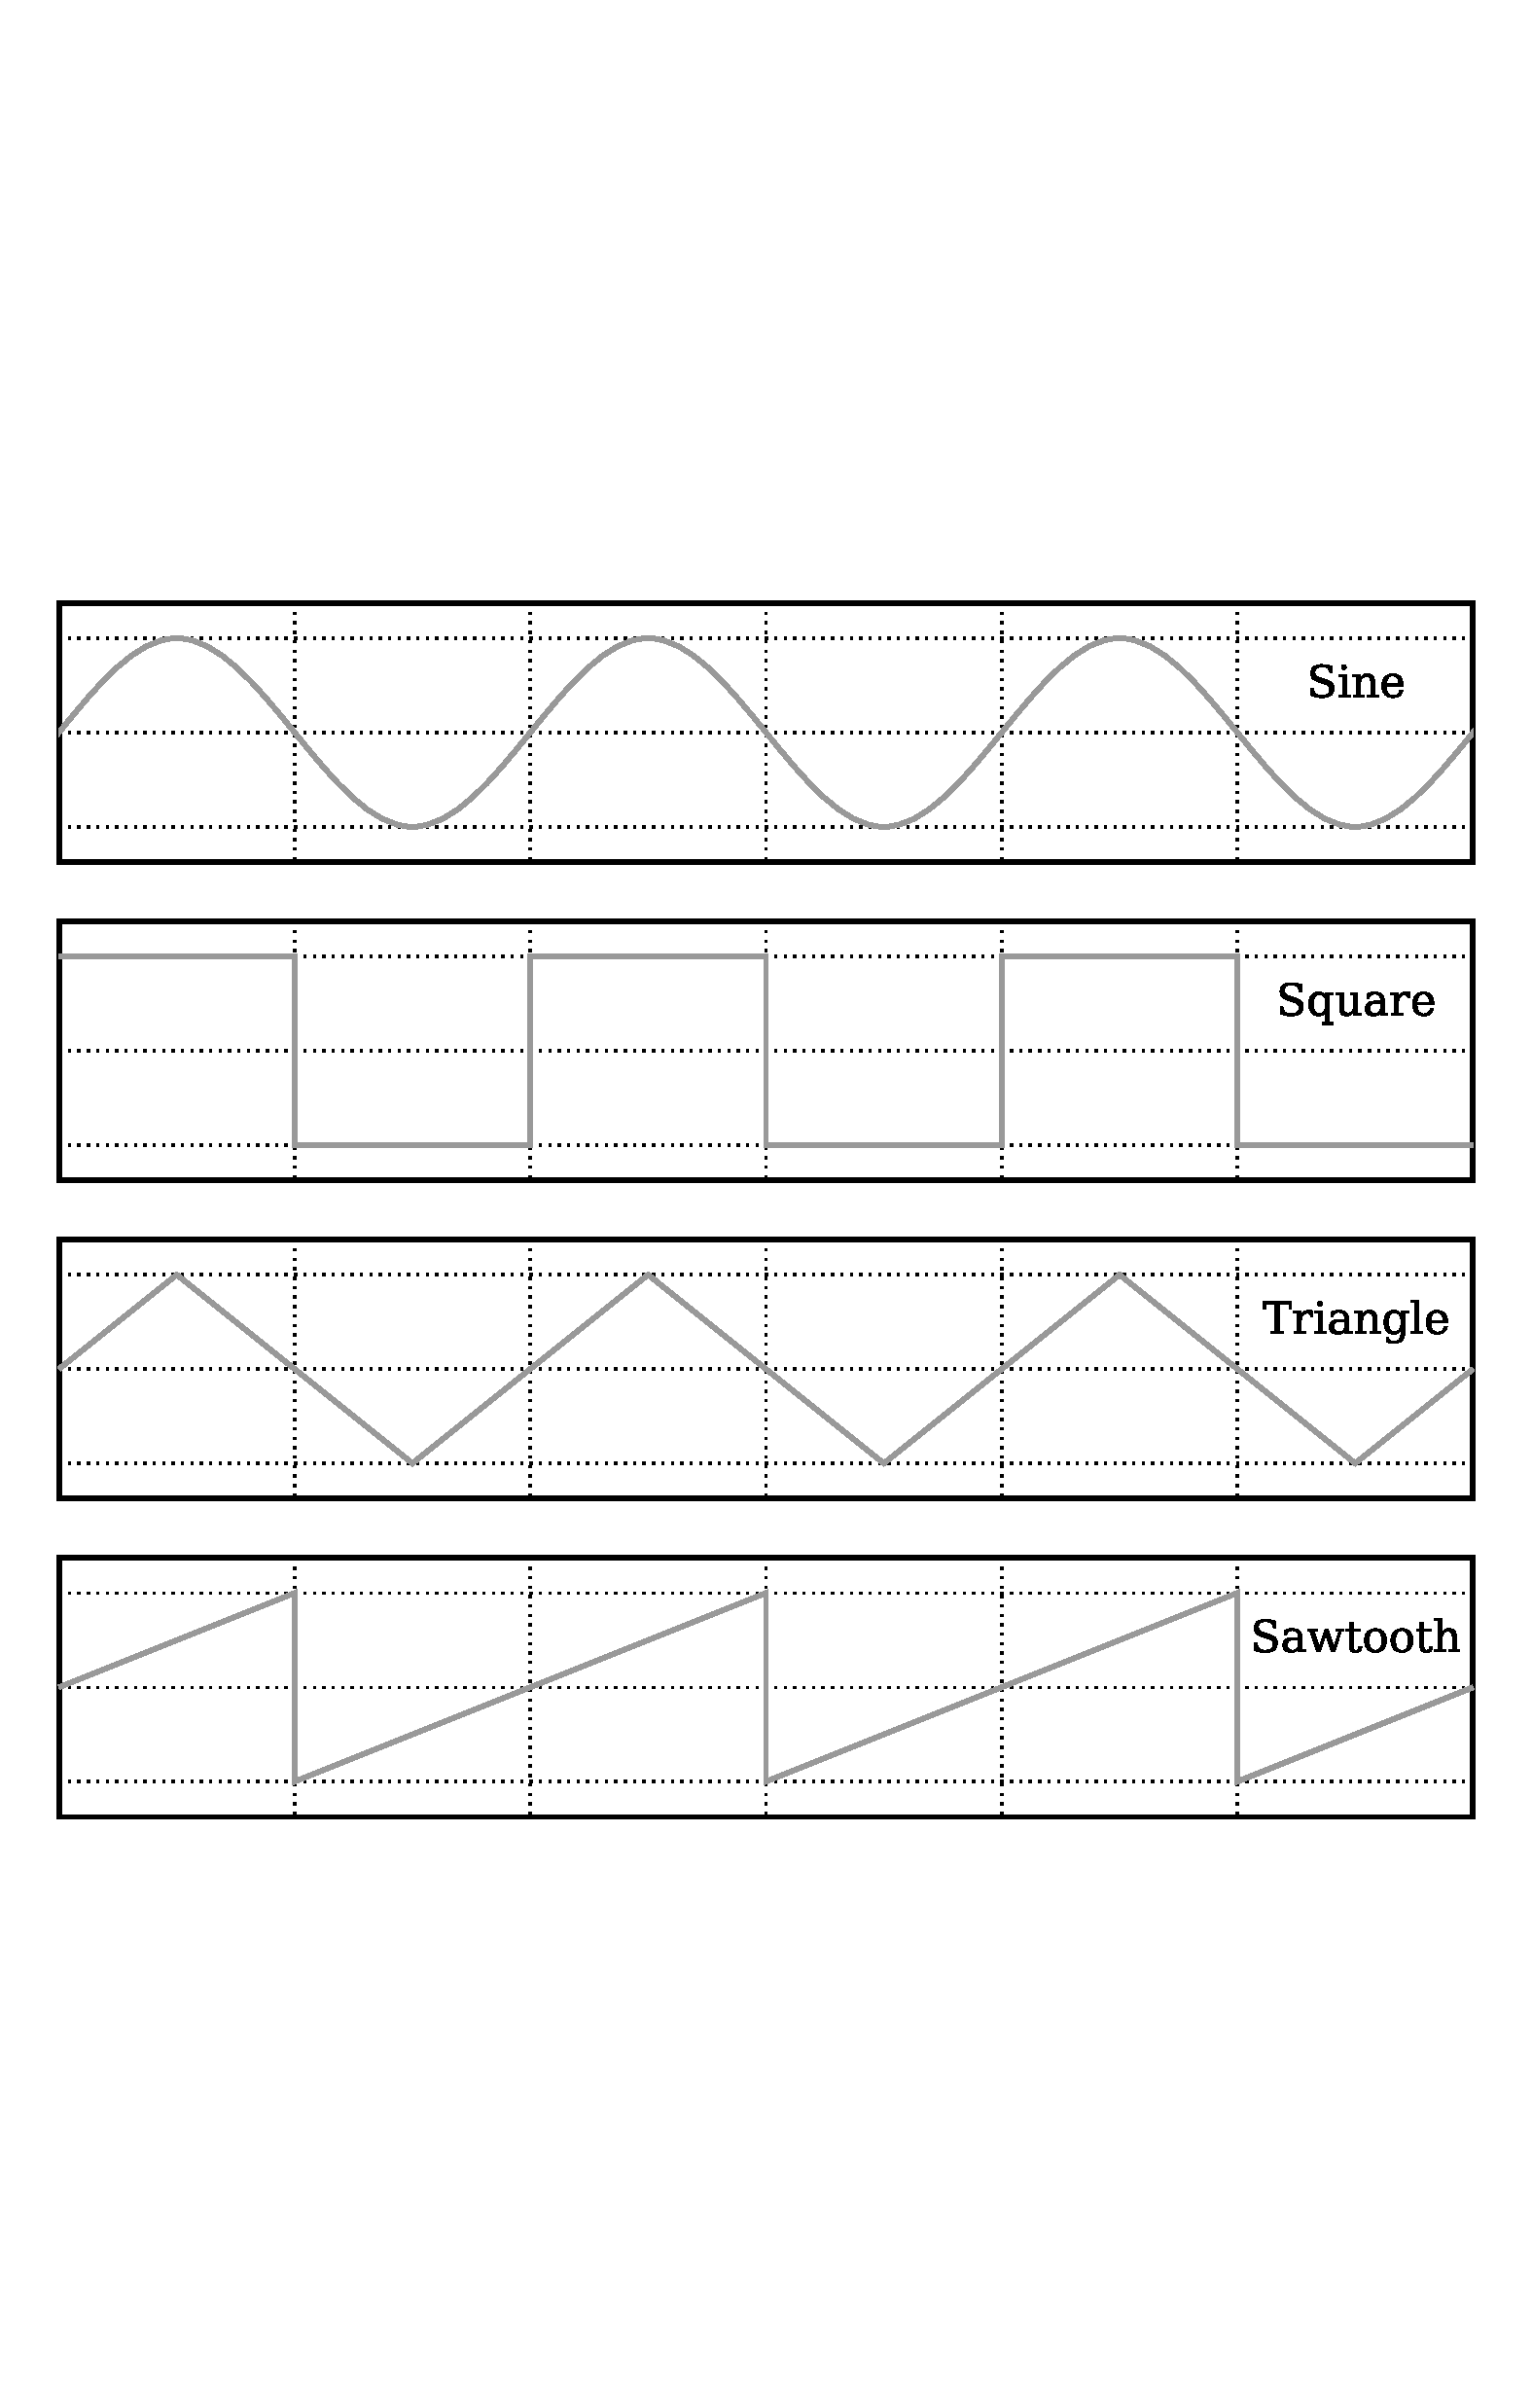
\includegraphics[width=0.8\linewidth]{images/Waveforms.pdf}}
  \caption[The different waveforms supported by the Web Audio API -
  \protect\newline{\small\url{http://en.wikipedia.org/wiki/File:Waveforms.svg} (20.02.2014)}
  \protect\newline{\small\emph{WikiMedia - User:Omegatron}}]{The different waveforms supported by the Web Audio API}
  \label{fig:waveforms}
\end{figure}

Oscillators in the Web Audio API support four different wave types which are shown in figure \reffigure{fig:waveforms} \cite{wilson2014webaudiospec}. The sine wave is the most classical wave that produces a pure note without overtones and is very uncommon to be used on its own in music programming but it is very often used to thicken the sound of other waves \cite[chapter: 2, Sine Wave]{cannAnalogSynthesis}. Square waves are often used for bass sounds and to create ``woody and reedy tones''\footnote{\cite[chapter: 2, Square Wave]{cannAnalogSynthesis}}. Triangle waves have a similar sound to sine waves but are more sharp. In early synthesizers, which were not capable of producing pure sine waves, triangle waves were used instead\footnote{\cite[chapter: 2, Triangle Wave]{cannAnalogSynthesis}}. Sawtooth waves have a bright sound and they are very commonly used for further sound shaping and filtering. Even after filtering, their unique sound will shine through the sculpted sound\footnote{\cite[chapter: 2, Sawtooth Wave]{cannAnalogSynthesis}}.

\begin{lstlisting}[language=JavaScript, caption=Playing a sound from an oscillator, label=lst:webaudiooscillator]
  var oscillator = context.createOscillator();
  // 0 -> sine; 1 -> square; 2 -> sawtooth; 3 -> triangle
  oscillator.type = 0;
  oscillator.frequency.value = 22000;
  oscillator.connect(context.destination);
  // start the oscillator
  oscillator.start(0);
\end{lstlisting}

As any other \code{AudioNode}, \code{Oscillators} are created from an \code{AudioContext} instance and they have to be wired into the node graph in order to create sounds (see \reflisting{lst:webaudiooscillator}). In addition to the above described waves (line 2f), an arbitrary wave can be created from a \code{Float32Array} and assigned to an oscillator object\footnote{\cite[createPeriodicWave]{wilson2014webaudiospec}}. In this way, developers could, e.g., add the missing pulse wave with a specific distribution of on- and off-time. A square wave is basically a pulse wave with a distribution of 50\%. The \code{frequency} property is of the special type \code{AudioParam} and needs to be set via the object's \code{value} property, instead of assigning it directly because \code{AudioParams} provide ways to exactly time parameter values (see \refchapter{sec:webaudio-timing}).

Line 4 is again a reminder that it is important to not keep the range of human hearing (20Hz to 20kHz) in mind. It creates a wave with a frequency of 22kHz which humans are not able to hear but the Web Audio API is still capable of creating these sounds. Frequencies that are lower than the `minimum' 20Hz come in handy when Low Frequency Oscillators (see \refchapter{sec:webaudio-synth}) are used to create new sounds, although their bare signal cannot be heard by humans.